%%#######################################################
%%#                   DHBW ULTIMATE                     #
%%#          LaTEX template for english papers          #
%%#           optimized for DHBW Stuttagrt              #
%%#                  computer science                   #
%%#                                                     #
%%#                                                     #
%%# based on: github.com/dhbw-horb/latexVorlageEnglisch #
%%#       by: t-kopp                                    #
%%#           (kevinkepp, ZaiLynch)                     #
%%#   author: Tobias Dreher, Yves Fischer (2011)        #
%%#                                                     #
%%#                                                     #
%%#     Marius Herget, info@herget.design, TINF14A      #
%%#######################################################

%%%%%%%%%%%%%%%%%%%%%%%%%%%%%%%%%%%%
%%%%%%% define your SETTINGS %%%%%%%
%%%%%%%%%%%%%%%%%%%%%%%%%%%%%%%%%%%%
\newcommand{\pdftitel}{DHBW-ULTIMATE}
\newcommand{\autor}{Marius Herget}
\newcommand{\arbeit}{Template LaTEX}
\newcommand{\version}{draft} % change to "final" to disable comments | "draft" shows notes/tbds/etc


%%%% Don't touch! %%%%
%
% Import settings for alle plugins / TEX
%
\documentclass[%
	pdftex,
	a4paper,
	%letterpaper,
	oneside,        % Oneside print
	12pt,           % Font size
	parskip=half,
%	headsepline,
	footsepline,
	plainfootsepline,
	abstracton,     % Abstract headline
	english,        % Translator																				% LANGUAGE
	%enabledeprecatedfontcommands, % enable old commands to use fancyhdr - NOT RECOMMENDED
%	listof=totoc
]{scrreprt}


% Include full other TEX documents --> via PDF
%\usepackage[subpreambles=true]{standalone}
%\usepackage{import}
\usepackage{standalone}

\renewcommand{\rmdefault}{phv} % Arial
\renewcommand{\sfdefault}{phv} % Arial
%Seitengroesse
\usepackage{fullpage}
\usepackage{pdfpages}
%Zeilenumbruch und mehr
\usepackage[activate]{microtype}

% Zeichencodierung
\usepackage[utf8]{inputenc}
\usepackage[T1]{fontenc}

% Zeilenabstand
\usepackage[onehalfspacing]{setspace}

% Index-Erstellung
\usepackage{makeidx}

% Lokalisierung (englische Sprache)
\usepackage[english]{babel}																						% LANGUAGE

% Anführungszeichen
\usepackage[babel,german=quotes]{csquotes}
%\usepackage[style=swiss]{csquotes}

% ca. 60-70 Zeichen pro Zeile pt12
\setlength\textheight{42\baselineskip}
\addtolength\textheight{\topskip}

%Kopf und Fußzeile
%\usepackage{fancyhdr}
\usepackage{scrlayer-scrpage}

% Spezielle Tabellenform fuer Deckblatt
\usepackage{longtable}
\setlength{\tabcolsep}{10pt} %Abstand zwischen Spalten
\renewcommand{\arraystretch}{1.5} %Zeilenabstand

% Grafiken
\usepackage{graphicx}
\usepackage{wrapfig}
\usepackage{subcaption} %To create subfigures
\usepackage{placeins} % FloatBarrier

% Biblatex
\usepackage[backend=bibtex,style=numeric]{biblatex}
\bibliography{content/literatur.bib}
\nocite{*}

% Mathematische Textsaetze
\usepackage{amsmath}
\usepackage{amssymb}

% Pakete um Textteile drehen zu können, oder eine Seite Querformat anzeigen kann.
\usepackage{lscape}

% Farben
\usepackage{color}
\definecolor{LinkColor}{rgb}{0,0,0.2}
\definecolor{ListingBackground}{rgb}{0.92,0.92,0.92}
\usepackage{xcolor}

% PDF Einstellungen
\usepackage[%
	pdftitle={\pdftitel},
	pdfauthor={\autor},
	pdfsubject={\arbeit},
	pdfcreator={pdflatex, LaTeX with KOMA-Script},
	pdfpagemode=UseOutlines, % Beim Oeffnen Inhaltsverzeichnis anzeigen
	pdfdisplaydoctitle=true, % Dokumenttitel statt Dateiname anzeigen.
	pdflang=eng % Sprache des Dokuments.																% LANGUAGE
]{hyperref}

% (Farb-)einstellungen für die Links im PDF
\hypersetup{%
	colorlinks=false, % Aktivieren von farbigen Links im Dokument
	linkcolor=LinkColor, % Farbe festlegen
	citecolor=LinkColor,
	filecolor=LinkColor,
	menucolor=LinkColor,
	urlcolor=LinkColor,
	bookmarksnumbered=true % Überschriftsnummerierung im PDF Inhalt anzeigen.
}

% Verschiedene Schriftarten
%\usepackage{goudysans}
%\usepackage{lmodern}
%\usepackage{libertine}
\usepackage{palatino}

% Hurenkinder und Schusterjungen verhindern
% http://projekte.dante.de/DanteFAQ/Silbentrennung
\clubpenalty=10000
\widowpenalty=10000
\displaywidowpenalty=10000

% Quellcode
\usepackage{listings}
\lstloadlanguages{Java}
\lstset{%
	language=Java,            % Sprache des Quellcodes
	numbers=left,            % Zeilennummern links
	stepnumber=1,            % Jede Zeile nummerieren.
	numbersep=5pt,           % 5pt Abstand zum Quellcode
	numberstyle=\tiny,       % Zeichengrösse 'tiny' für die Nummern.
	breaklines=true,         % Zeilen umbrechen wenn notwendig.
	breakautoindent=true,    % Nach dem Zeilenumbruch Zeile einrücken.
	postbreak=\space,        % Bei Leerzeichen umbrechen.
	tabsize=2,               % Tabulatorgrösse 2
	basicstyle=\ttfamily\footnotesize, % Nichtproportionale Schrift, klein für den Quellcode
	showspaces=false,        % Leerzeichen nicht anzeigen.
	showstringspaces=false,  % Leerzeichen auch in Strings ('') nicht anzeigen.
	extendedchars=true,      % Alle Zeichen vom Latin1 Zeichensatz anzeigen.
	captionpos=b,            % sets the caption-position to bottom
	backgroundcolor=\color{ListingBackground}, % Hintergrundfarbe des Quellcodes setzen.
	escapechar=@		 % Escape to use bold
}

% Glossar
\usepackage[
	nonumberlist, %keine Seitenzahlen anzeigen
	acronym,      %ein Abkürzungsverzeichnis erstellen
	%section,     %im Inhaltsverzeichnis auf section-Ebene erscheinen
	toc,          %Einträge im Inhaltsverzeichnis
]{glossaries}

% Fussnoten
\usepackage[perpage, hang, multiple, stable]{footmisc}

% Overloading Macros
\usepackage{xparse}

% Plotting diagramms
\usepackage{tikz} % To generate the plot from csv
\usepackage{flowchart}

\usepackage{pgfplots}
\usepackage{pgfplotstable}
\pgfplotsset{compat=1.10}
\usepgfplotslibrary{fillbetween}
\usepgfplotslibrary{groupplots}
\usetikzlibrary{pgfplots.groupplots}
\usetikzlibrary{patterns}
 % zoom in
\usetikzlibrary{spy,backgrounds}

% use tikz also to create flowcharts
\usetikzlibrary{arrows}
\usetikzlibrary{shapes.geometric, arrows}
	% Define block styles 1
	\tikzstyle{own:process} = [rectangle, minimum width=3cm, minimum height=1cm, text centered, text width=3.5cm, draw=black, fill=orange!30]
	\tikzstyle{own:decision} = [diamond, minimum width=3cm, minimum height=1cm, text centered, draw=black, fill=green!30]
	\tikzstyle{own:io} = [trapezium, trapezium left angle=70, trapezium right angle=110, minimum width=3cm, minimum height=1cm, text centered, draw=black, fill=blue!30]
	\tikzstyle{own:startstopsmall} = [rectangle, rounded corners, minimum width=3cm, text width=3.5cm, minimum height=1cm,text centered, draw=black, fill=red!30]
	\tikzstyle{own:startstop} = [rectangle, rounded corners, minimum width=3cm, minimum height=1cm,text centered, draw=black, fill=red!30]
	\tikzstyle{own:arrow} = [thick,->,>=stealth]

% DEBUG wrong float
%\usepgfplotslibrary{external}
%\tikzexternalize[prefix=diagrams/rendered/]
%\tikzexternalize

% Aufzaehlungen
\usepackage{enumitem}

% Tables
%\usepackage{tabularx}
\usepackage{ltablex} % mix out of tabularx and longtable
\usepackage{multirow}

% Better References
\usepackage{cleveref}

% Display folder/file structures
\usepackage{dirtree}

% Titel, Autor und Datum
\title{\titel}
\author{\autor}
\date{\datum}

% Abstand 2,5cm allseits
\usepackage[
  top = 2.5cm,
  bottom = 2.5cm,
  left = 2.5cm,
  right = 2.50cm]{geometry}

\pgfplotsset{
    discard if not/.style 2 args={
        x filter/.code={
            \edef\tempa{\thisrow{#1}}
            \edef\tempb{#2}
            \ifx\tempa\tempb
            \else
                \def\pgfmathresult{inf}
            \fi
        }
    }
}

\usepackage{xkvltxp}
\usepackage[\version, layout={inline,index}, singleuser]{fixme}
\fxsetup{envlayout=plain}
\renewcommand\fixmeindexname{hello}
\renewcommand\@fxnotekey{***a}
\renewcommand\@fxwarningkey{***b}
\renewcommand\@fxerrorkey{***c}
\renewcommand\@fxfatalkey{***d}
\FXLayoutIndex {htypei}{hnotei}{hauthor i}
\renewcommand*\FXLayoutIndex[3]{%
	\iffx@mode@multiuser%
	\index{***@\fixmeindexname:%
	\@nameuse{@fx#1key}@\fxnotesname{#1}:%
	\@nameuse{thefx#1count}: #3: #2}%
	\index{***#3@\fixmeindexname{} (#3):%
	\@nameuse{@fx#1key}@\fxnotesname{#1}:%
	\@nameuse{thefx#1count}: #2}%
	\else%
	\index{***@\fixmeindexname:%
	\@nameuse{@fx#1key}@\fxnotesname{#1}:%
	\@nameuse{thefx#1count}: #2}%
	\fi}
\@fxlayout@index
\FXRegisterLayout{index}{\FXLayoutIndex}

% Appendix
\usepackage[toc,page]{appendix}

% Single label
% example: \singlelabel{extra}{\caption{An image}}
\makeatletter
\newcommand{\singlelabel}[2]{%
  \ifcsname singlelabel#1\endcsname
    % the file has already been read
    \@namedef{the\@captype}{\ref{#1}}%
    #2%
  \else
    #2\label{#1}
    \global\@namedef{singlelabel#1}{}%
  \fi
}
\makeatother

% Print CSV as tables
\usepackage{csvsimple}
\usepackage{adjustbox}

% print PERF output --> txt
\usepackage{verbatim}
%\usepackage{fancyvrb}
%% redefine \VerbatimInput
%\RecustomVerbatimCommand{\VerbatimInput}{VerbatimInput}%
%{fontsize=\footnotesize,
% %
% frame=lines,  % top and bottom rule only
% framesep=2em, % separation between frame and text
% rulecolor=\color{Gray},
% %
% label=\fbox{\color{Black}data.txt},
% labelposition=topline,
% %
%% commandchars=|\(\), % escape character and argument delimiters for
%                      % commands within the verbatim
% commentchar=*        % comment character
%}

%PDF INCLUDE
\usepackage{pdfpages}

\IfFileExists{ownFrameworks.tex}{\input{ownFrameworks}}{}
%%%%%%%%%%%%%%%%%%%%%%

% Ab jetzt können auch Umlaute verwendet werden
%%%%%%%%%%%%%%%%%%%%%%%%%%%%%%%%%%%%
%%%%%%%%%% other SETTINGS %%%%%%%%%%
%%%%%%%%%%%%%%%%%%%%%%%%%%%%%%%%%%%%
\newcommand{\titel}{How to build your own Death Star based on your personal 3D printer}
\newcommand{\untertitel}{... and why there will be unicorns}
\newcommand{\matrikelnr}{1337}
\newcommand{\kurs}{TINF14A}
\newcommand{\datumAbgabe}{January 4242}
\newcommand{\firma}{Todesstern GmBH}
\newcommand{\firmenort}{Stuttgart, GER}
\newcommand{\abgabeort}{Stuttgart}
\newcommand{\abschluss}{Bachelor of Science}
\newcommand{\studiengang}{Applied Unicorn Science}
\newcommand{\dhbw}{Stuttgart}
\newcommand{\betreuer}{Darth Vader}
\newcommand{\gutachter}{Luke Skywalker}
\newcommand{\zeitraum}{3rd PE}
\newcommand{\jahr}{2016}

\newcommand{\confidental}{Empire CONFIDENTAL} % remark right lower corner

%%%%%%%%%%%%%%%%%%%%%%%%%%%%%%%%%%%%%%%%%%%%%%%%%%%%%%%%%%%%%%%%%%%%%%%%%%%%%%%%%%%%%%%%
%%%%%%%%%%%%%%%%%%%%%%%%%%%%%%%%%%%%%%%%%%%%%%%%%%%%%%%%%%%%%%%%%%%%%%%%%%%%%%%%%%%%%%%%
%%% You don't need to work here if you are not familiar with latex and this template %%%
%%%%%%%%%%%%%%%%%%%%%%%%%%%%%%%%%%%%%%%%%%%%%%%%%%%%%%%%%%%%%%%%%%%%%%%%%%%%%%%%%%%%%%%%
%%%%%%%%%%%%%%%%%%%%%%%%%%%%%%%%%%%%%%%%%%%%%%%%%%%%%%%%%%%%%%%%%%%%%%%%%%%%%%%%%%%%%%%%
%%%%%%%%%%%%%%%%%%%%%%%%%%%%%%%%%%%%%%%%%%%%%%%%%%%%%%%%%%%%%%%%%%%%%%%%%%%%%%%%%%%%%%%%
%%%%%%%%%%%%%%%%%%%%%%%%%%%%%%%%%%%%%%%%%%%%%%%%%%%%%%%%%%%%%%%%%%%%%%%%%%%%%%%%%%%%%%%%
%%%%%%%%%%%%%%%%%%%%%%%%%%%%%%%%%%%%%%%%%%%%%%%%%%%%%%%%%%%%%%%%%%%%%%%%%%%%%%%%%%%%%%%%
%%%%%%%%%%%%%%%%%%%%%%%%%%%%%%%%%%%%%%%%%%%%%%%%%%%%%%%%%%%%%%%%%%%%%%%%%%%%%%%%%%%%%%%%
%%%%%%%%%%%%%%%%%%%%%%%%%%%%%%%%%%%%%%%%%%%%%%%%%%%%%%%%%%%%%%%%%%%%%%%%%%%%%%%%%%%%%%%%
%%%%%%%%%%%%%%%%%%%%%%%%%%%%%%%%%%%%%%%%%%%%%%%%%%%%%%%%%%%%%%%%%%%%%%%%%%%%%%%%%%%%%%%%
\rofoot*{\confidental}

%% NEW commands for better workfloe
\newcommand{\impmark}{\strut\vadjust{\domark}}
\newcommand{\domark}{%
	\vbox to 0pt{
		\kern-\dp\strutbox
		\smash{\llap{*\kern1em}}
		\vss
	}%
}
\newcommand{\impquest}{\strut\vadjust{\doquest}}
\newcommand{\doquest}{%
	\vbox to 0pt{
		\kern-\dp\strutbox
		\smash{\llap{?\kern2em}}
		\vss
	}%
}
% TBD
\newcommand{\tbd}[1][null]{
	\ifthenelse{\equal{#1}{null}}
	{\fxwarning[]{\textit{\impmark\color{orange}(TBD)} }}
	{\fxnote[]{\textit{\impmark\color{orange}#1}}}
}
\newcommand{\todo}[1][null]{
	\ifthenelse{\equal{#1}{null}}
	{\fxwarning[]{\textit{\impmark\color{orange}(TBD)} }}
	{\fxnote[]{\textit{\impmark\color{orange}#1}}}
}

\newcommand{\question}[1][???]{\fxfatal[]{\impquest\color{red}#1}}
\let\origdoublepage\cleardoublepage
\renewcommand{\cleardoublepage}{%
  \clearpage
  {\pagestyle{empty}\origdoublepage}%
}

\cleardoublepage
\makeglossaries
%
% vorher in Konsole folgendes aufrufen: 
%	makeglossaries makeglossaries dokumentation.acn && makeglossaries dokumentation.glo
%

%
% Abkürzungen --> referenz, name, beschreibung
% Aufruf mit \gls{...} oder Kurzform mit \acrshort{...}
%

\newacronym{DHBW}{DHBW}{Duale Hochschule Baden Württemberg}
\newacronym{DV}{DV}{\gls{Vader}}


%
% Glossareintraege --> referenz, name, beschreibung
% Aufruf mit \gls{...}
%
\newglossaryentry{Vader}{name={Darth Vader},plural={Darth Vaders},description={The best Lord of all time.}}

\glsaddall


\begin{document}
	% Deckblatt
	\begin{spacing}{1}
		\cleardoublepage
		\begin{titlepage}
	\begin{longtable}{p{.55\textwidth} p{.85\textwidth}}
		{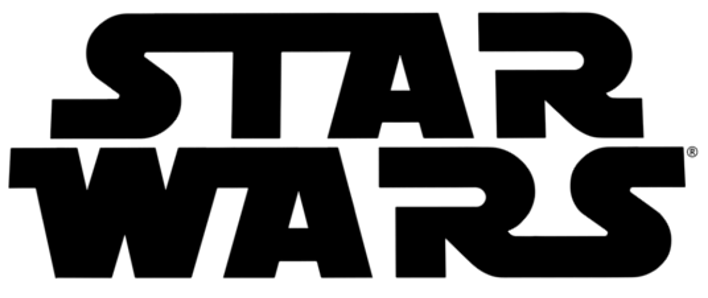
\includegraphics[height=1.6cm]{images/logo.png}} &
		{
\includegraphics[height=2.6cm]{images/dhbw.png}}
	\end{longtable}
	\enlargethispage{20mm}
	\begin{center}
		\ifthenelse{\equal{\version}{draft}}
		{\textit{ *** DRAFT VERSION *** \\{\tiny \today \\}}}
		{\vspace*{12mm}}
		{\LARGE\textbf{ \titel }}\\
		\vspace*{4mm}   {\large \untertitel}\\
		\vspace*{12mm}	{\large\textbf{ \arbeit}}\\
		\vspace*{8mm}  	for the\\
		\vspace*{3mm} 	{\textbf{ \abschluss}}\\
		\vspace*{12mm}	at Course of Studies \studiengang\\
		\vspace*{3mm} 	at the Cooperative State University \dhbw\\
		\vspace*{12mm}	by\\
		\vspace*{3mm} 	{\large\textbf{ \autor}}\\
		\vspace*{12mm}	\datumAbgabe\\
	\end{center}
	\vfill
	\begin{spacing}{1.2}
		\begin{tabbing}
			mmmmmmmmmmmmmmmmmmmmmmmmmm     \= \kill
			\textbf{Time of Project}  \>  \zeitraum\\
			\textbf{Student ID, Course}  \>  \matrikelnr, \kurs\\
			\textbf{Company}      \>  \firma, \small{\textit{\firmenort}}\\
			\textbf{Supervisor in the Company}              \>  \betreuer\\
			\textbf{Reviewer}             \>  \gutachter
		\end{tabbing}
	\end{spacing}
	\begin{flushright}
		\copyright{} \jahr
	\end{flushright}
\end{titlepage}

		\cleardoublepage
		\listoffixmes % todos
	\end{spacing}
	\newpage

	\renewcommand{\thepage}{\Roman{page}}
	\setcounter{page}{1}

	% Declaration
	\cleardoublepage
	\thispagestyle{empty}

\section*{Author's declaration}
% Seite 8
% http://studium.ba-bw.de/fileadmin/media/allgemein/bestimmungen/btechnik/richtlinien/Richtlinien_Praxismodule_Studien_und_Bachelorarbeiten_2011.pdf
\vspace*{2em}
Unless otherwise indicated in the text or references, or acknowledged above, this thesis is entirely the product of my own scholarly work. This thesis has not been submitted either in whole or part, for a degree at this or any other university or institution. This is to certify that the printed version is equivalent to the submitted electronic one.
\vspace{3em}

\abgabeort, \datumAbgabe
\vspace{4em}

\rule{6cm}{0.4pt}\\
\autor



	\newpage

	% Abstract
	\cleardoublepage
	\pagestyle{empty}

\renewcommand{\abstractname}{Zusammenfassung}
\begin{abstract}
Ein Abstract ist eine prägnante Inhaltsangabe, ein Abriss ohne
Interpretation und Wertung einer wissenschaftlichen Arbeit. In DIN
1426 wird das (oder auch der) Abstract als Kurzreferat zur
Inhaltsangabe beschrieben.

\begin{description}
\item[Objektivität] soll sich jeder persönlichen Wertung enthalten
\item[Kürze] soll so kurz wie möglich sein
\item[Genauigkeit] soll genau die Inhalte und die Meinung der Originalarbeit wiedergeben
\end{description}

Üblicherweise müssen wissenschaftliche Artikel einen Abstract
enthalten, typischerweise von 100-150 Wörtern, ohne Bilder und
Literaturzitate und in einem Absatz.

Quelle \url{http://de.wikipedia.org/wiki/Abstract} Abgerufen 07.07.2011
\end{abstract}


\renewcommand{\abstractname}{Summary}
\begin{abstract}
An abstract is a brief summary of a research article, thesis, review,
conference proceeding or any in-depth analysis of a particular subject
or discipline, and is often used to help the reader quickly ascertain
the paper's purpose. When used, an abstract always appears at the
beginning of a manuscript, acting as the point-of-entry for any given
scientific paper or patent application. Abstracting and indexing
services for various academic disciplines are aimed at compiling a
body of literature for that particular subject.

The terms précis or synopsis are used in some publications to refer to
the same thing that other publications might call an "abstract". In
management reports, an executive summary usually contains more
information (and often more sensitive information) than the abstract
does.

Quelle: \url{http://en.wikipedia.org/wiki/Abstract_(summary)}

\end{abstract}

	\newpage

	\pagestyle{scrheadings}

	% Table of contents
	\begin{spacing}{1}
		\cleardoublepage
		\pagenumbering{Roman}
		\setcounter{tocdepth}{3}
		\tableofcontents
		\cleardoublepage
	\end{spacing}

	% Abbildungsverzeichnis
	\cleardoublepage
	\phantomsection \label{listoffig}\addcontentsline{toc}{chapter}{\listfigurename}
	\listoffigures

	% Tabellenverzeichnis
	\cleardoublepage
	\phantomsection \label{listoftab}\addcontentsline{toc}{chapter}{\listtablename}
	\listoftables

	% Quellcodeverzeichnis
	\cleardoublepage
	\phantomsection \label{listoflist}\addcontentsline{toc}{chapter}{List of \lstlistlistingname}
	\lstlistoflistings

	% Abkürzungsverzeichnis
	% vorher in Konsole folgendes aufrufen:
	%	makeglossaries makeglossaries dokumentation.acn && makeglossaries dokumentation.glo
	\cleardoublepage
	%\phantomsection
	\printglossary[type=\acronymtype]
	% Glossar
	\cleardoublepage
	%\phantomsection
	\printglossary[style=altlist,title=Glossary]

	\cleardoublepage \clearpage
	\pagenumbering{arabic}
	% Inhalt
	\setstretch{1,5} % 1,5zeilig
	\patchcmd{\chapter}
	  {\clearpage}
	  {\cleardoublepage}
	  {}
	  {}
	   % contents file is generated by make
	  \IfFileExists{.TEX/contents.tex}
	    {\input{.TEX/contents}}
	    {NO CONTENTS FILE AVAILABLE.\\
	    \textbf{Please render with makefile or create a file like the following:}\\
	    \textbackslash\{content/main/filename1\}\\
	    \textbackslash\{content/main/filename2\}\\
	    }
	\setstretch{1}

	% Anhang
	\clearpage
	\pagenumbering{roman}

	% Literaturverzeichnis
	\cleardoublepage
	\phantomsection \label{listoflit}
	\addcontentsline{toc}{chapter}{Bibliography}
	\printbibliography


	\cleardoublepage
	% Appendix
	\IfFileExists{.TEX/appendices.tex}
	{
		\captionsetup{list=no}
		%\addtocontents{lof}{\protect\setcounter{tocdepth}{0}} %trick to dont show appendicies in table of contents/figures/...

		\begin{appendices}\label{appendices}
			\lofoot*{Appendices}
			\cleardoublepage
			\pagenumbering{arabic}
			\renewcommand{\thesubsection}{\Alph{subsection}}
			\input{.TEX/appendices.tex}
		\end{appendices}
	}
	{}
\end{document}
